\documentclass[12pt]{article}

% Math and symbol packages
\usepackage{amsmath}
\usepackage{amssymb}
\usepackage{derivative}

% Figure Packages
\usepackage{graphicx}
\usepackage{wrapfig}
\usepackage{epstopdf}
\usepackage{float}
\usepackage{subfigure}

% Formatting and Random Text Generation
\usepackage{inputenc}
\usepackage[left=2.54cm,right=2.54cm,top=2.54cm,bottom=2.54cm]{geometry}
\usepackage{lipsum}

% Header and indent packages
\usepackage{fancyhdr}
\usepackage{indentfirst}

% Create Title Section
\title{Rotational Kinetic Energy}
\author{Trevor Swan \\
Department of Physics, Case Western Reserve University \\
Cleveland, OH 44016-7079}
\date{}

% Create paragraph formatting
%\setlength{\parindent}{3em}

% Actual Lab content
\begin{document}
\pagestyle{fancy}
\fancyhf{}

% Load the title
\maketitle
\thispagestyle{fancy}
\renewcommand{\headrulewidth}{0pt}

% Set up Footers
\fancyfoot[L]{Trevor Swan}
\fancyfoot[C]{\thepage}
\fancyfoot[R]{Rotational Kinetic Energy}

% Abstract section of Report
\section{Abstract}
\lipsum[1]

% Introduction and Thoery
\section{Introduction and Theory}
\lipsum[2]

% Procedure
\section{Experimental Procedure}
\lipsum[3]

% Results and Analysis
\section{Results and Analysis}
\lipsum[4]

% Conclusion
\section{Conclusion}
\lipsum[6]

\subsection{Acknowledgments}
I would like to thank Adi Mallik, CWRU Department of Physics, for his help in obtaining the experimental data, preparing the figures, and checking my calculations.

\subsection{References}
\begin{enumerate}
    \item Driscoll, D., General Physics I: Mechanics Lab Manual, “Inclined Plane,” CWRU Bookstore, 2014.
\end{enumerate}

\section{Appendix}\
% Display the massless plot 

\begin{figure} [p]
    \begin{subfigure}
        \centering
        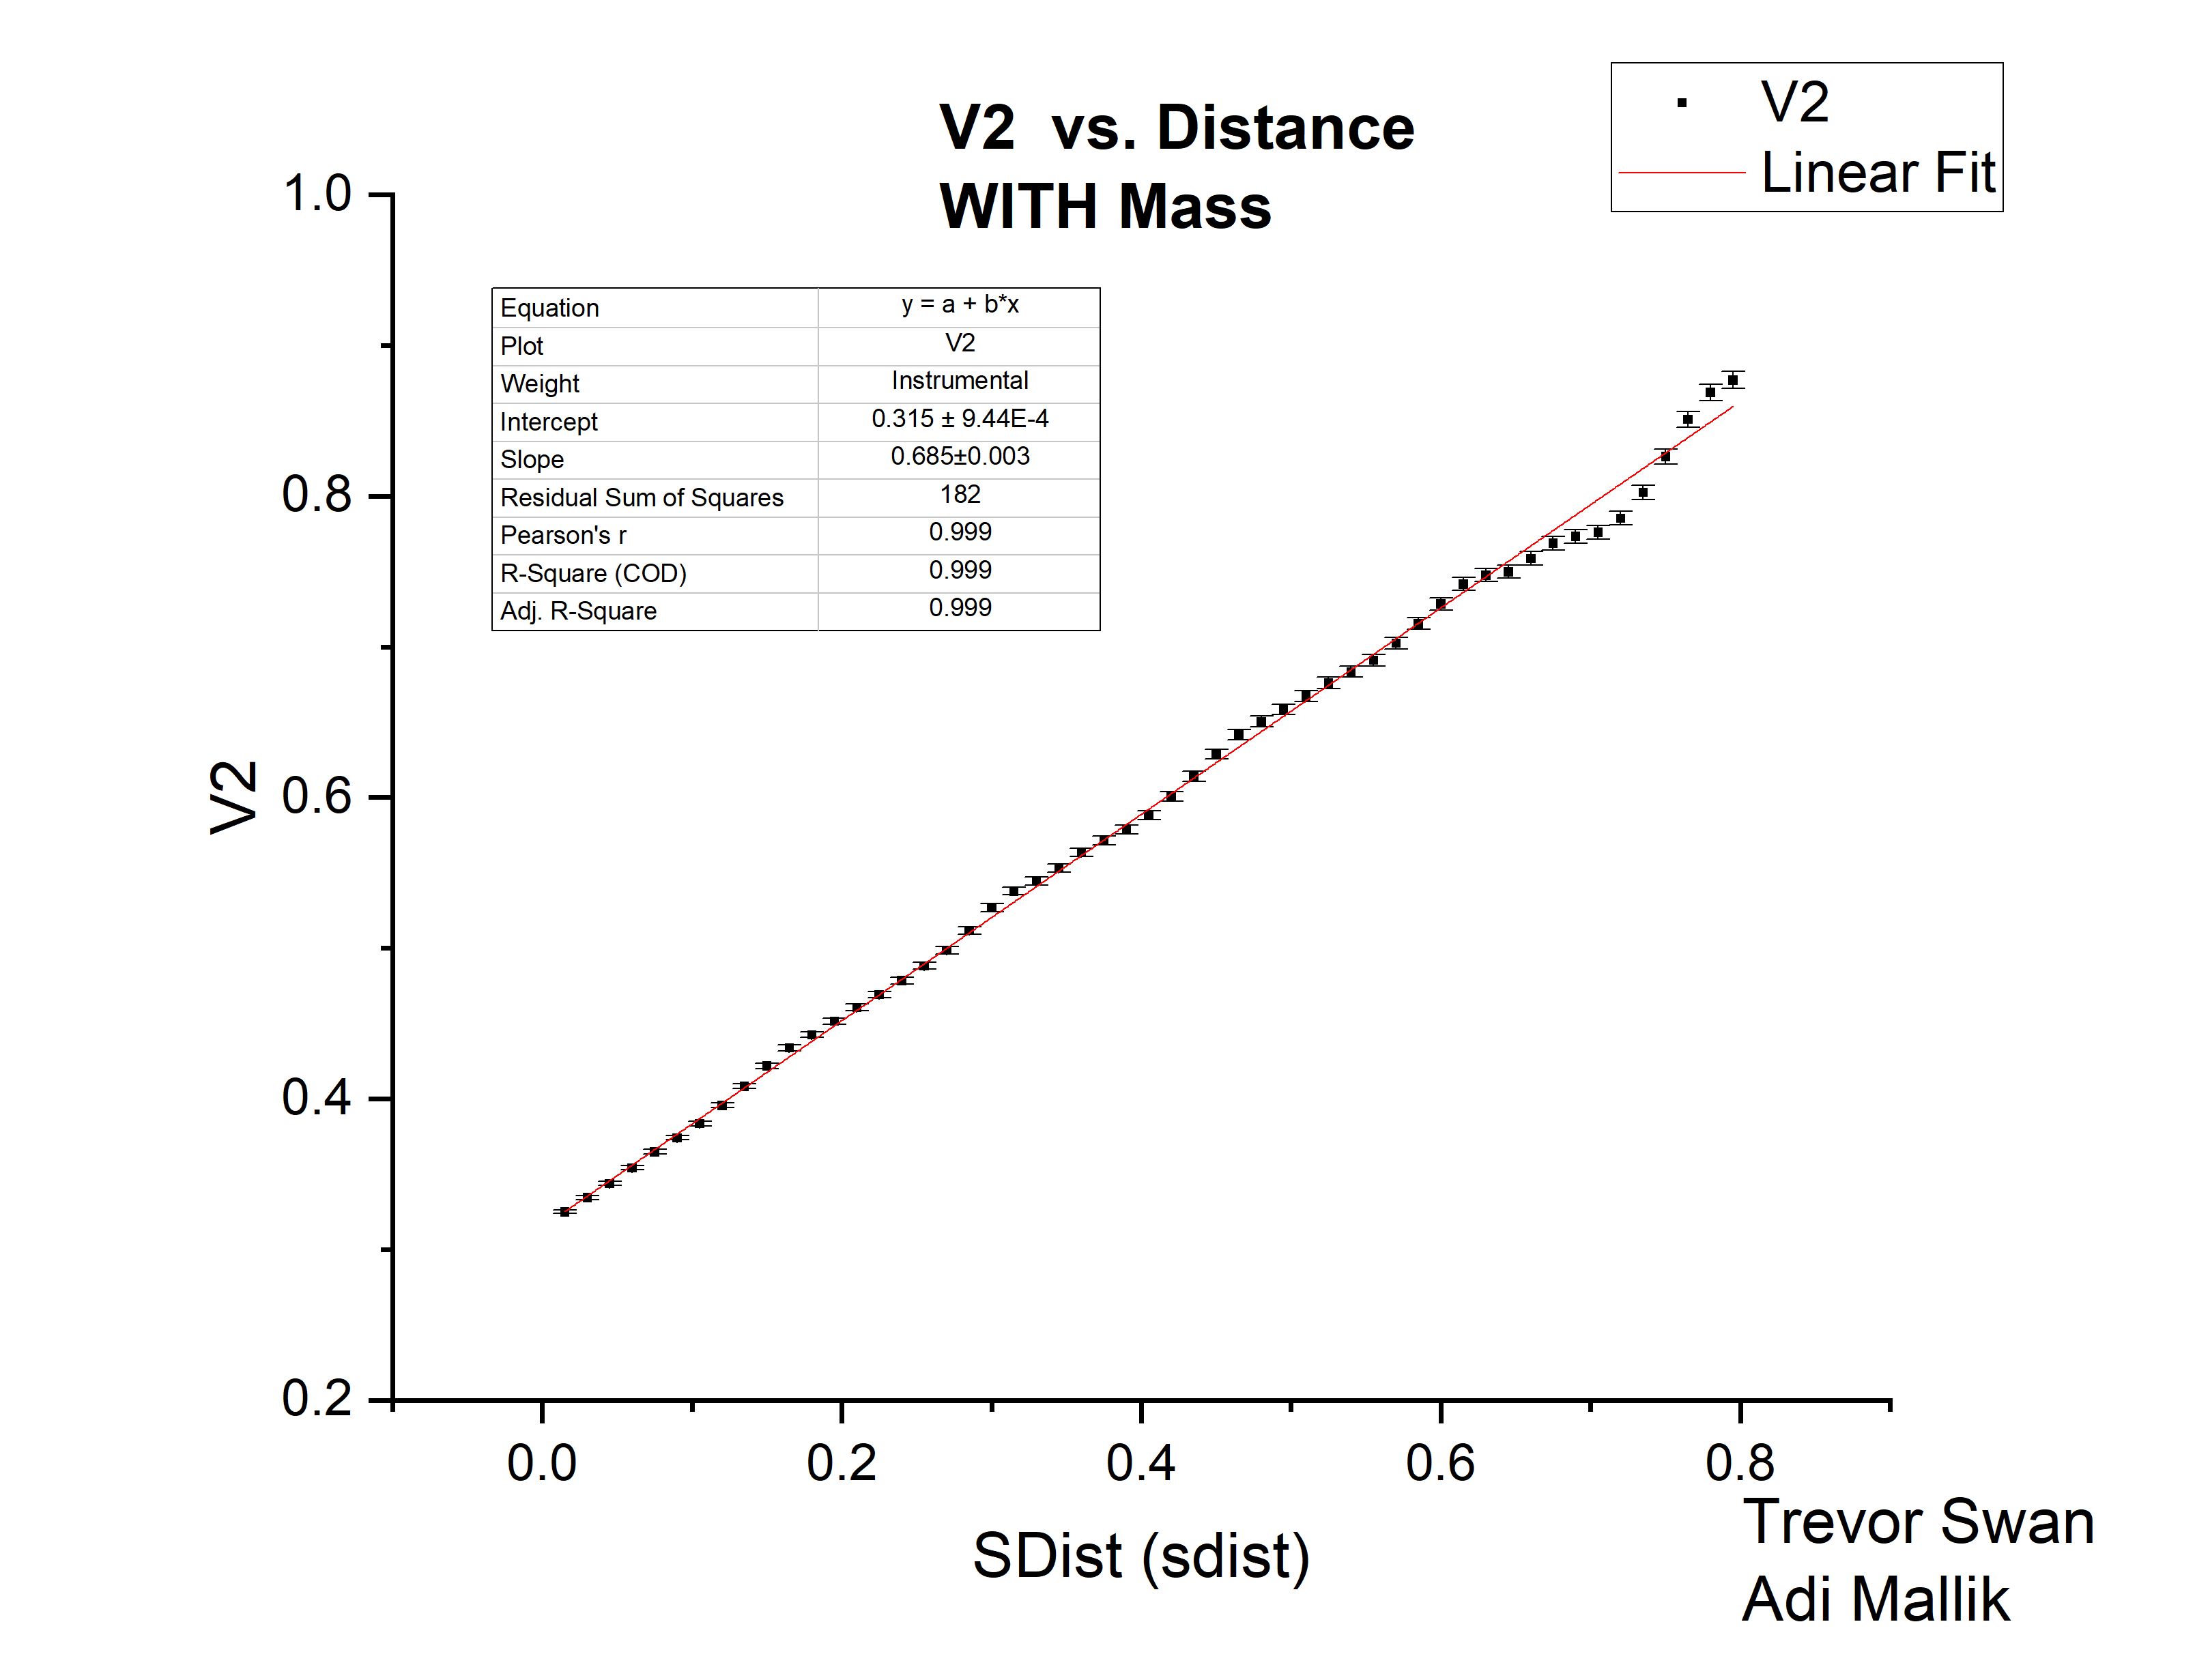
\includegraphics[width=0.8\textwidth]{RKE_withMass.png}
        \caption{$v^2$ vs. $y$ with mass}
        \label{Massed Plot}
    \end{subfigure}
    \begin{subfigure}
        \centering
        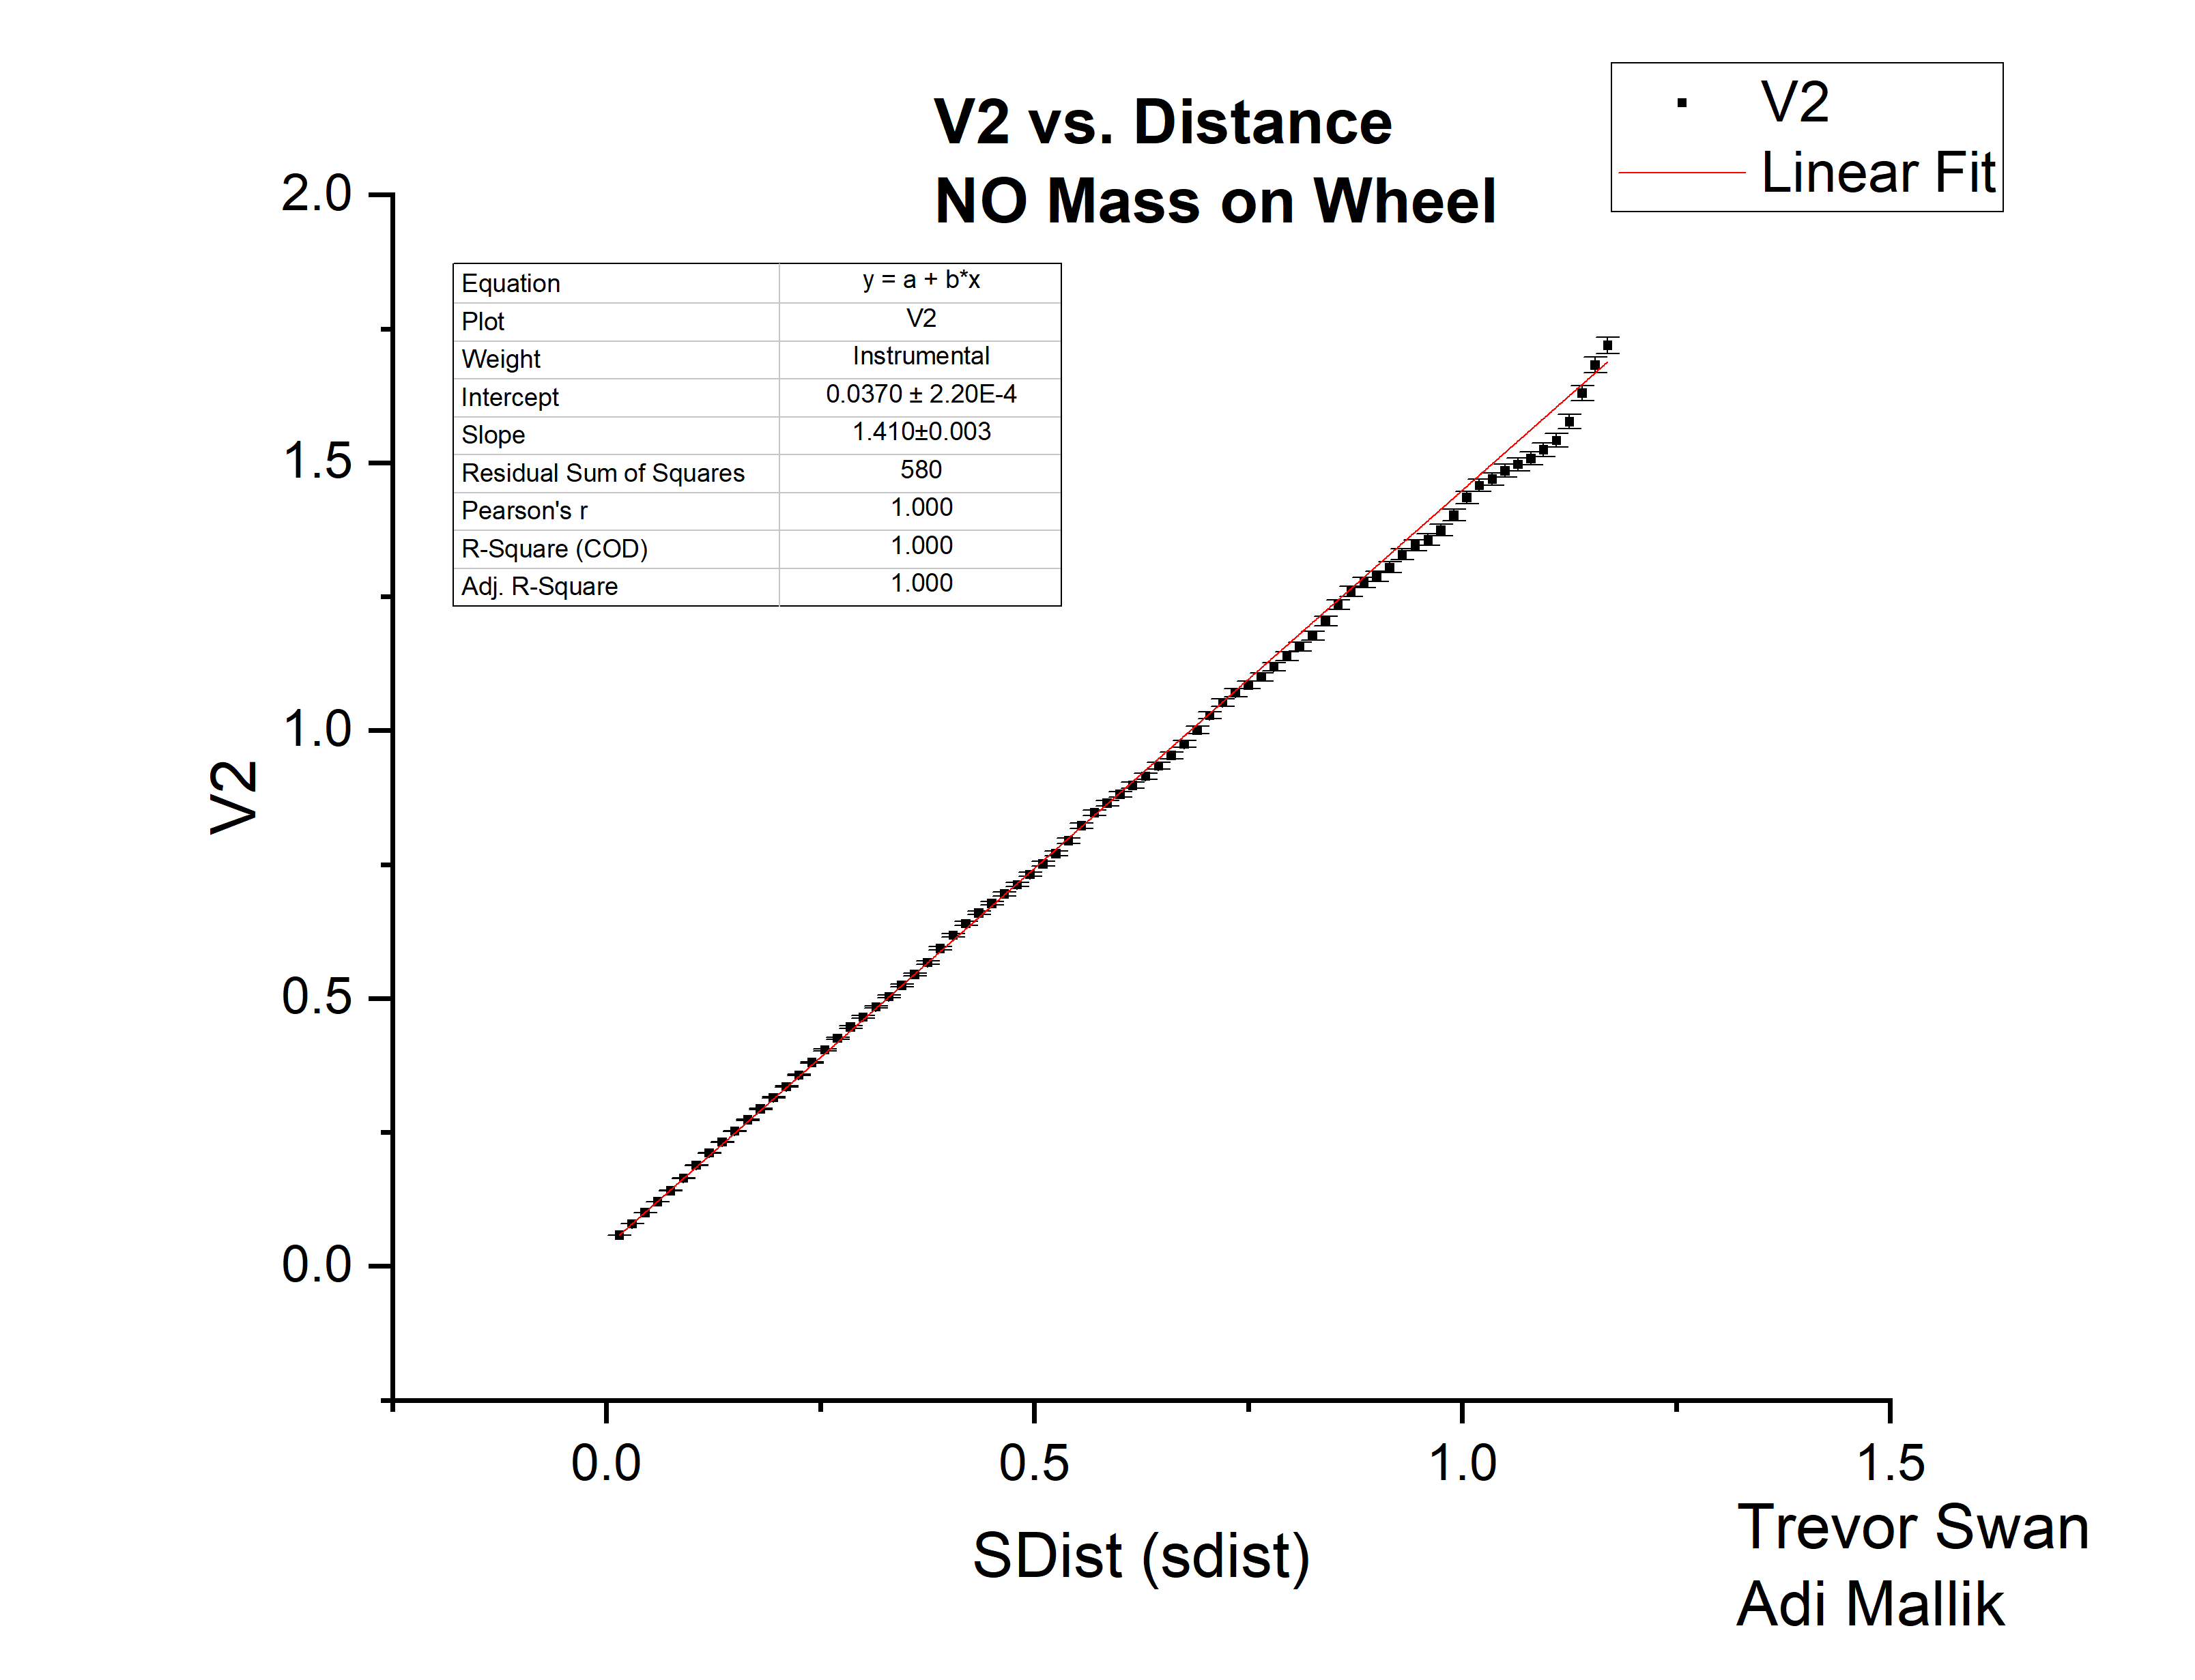
\includegraphics[width=0.8\textwidth]{RKE_noMass.png}
        \caption{$v^2$ vs. $y$ with no mass}
        \label{Massless Plot}
    \end{subfigure}
    
\end{figure}
\end{document}
